\documentclass[uplatex]{jsarticle}
\usepackage{bm}
\usepackage{braket}
\usepackage{amsmath,amssymb}
\usepackage[dvipdfmx]{graphicx}

\begin{document}
\section{EMアルゴリズム}
対数尤度$\log q(\bm{X}; \bm{\theta})$の下界は以下のようになり,これを$f$とおく.
\begin{eqnarray}
\label{em_objective}
f(\bm{X}; \bm{\theta}) = \int q(\bm{Z})\log p(\bm{X}, \bm{Z}; \bm{\theta}) d\bm{Z}
\end{eqnarray}
この下界を最大化するパラメータ$\bm{\pi}, \bm{\mu}, \bm{\Lambda}$を求める.まず,

$$q(\bm{Z}) = \prod_{n=1}^N \prod_{k=1}^K \gamma_{nk}^{z_{nk}}$$
$$p(\bm{X},  \bm{Z}; \bm{\theta}) = \prod_{n=1}^N \prod_{k=1}^K (\pi_k N(\bm{x}_n \mid \bm{\mu}_k, \bm{\Lambda}_k^{-1}))^{z_{nk}}$$
であり,これを式(\ref{em_objective})に代入して整理すると,次のようになる.
\begin{eqnarray}
\label{em_tidy}
f(\bm{X}; \bm{\theta}) &=& \int \prod_{n=1}^N \prod_{k=1}^K \gamma_{nk}^{z_{nk}} \log \prod_{n=1}^N \prod_{k=1}^K (\pi_k N(\bm{x}_n \mid \bm{\mu}_k, \bm{\Lambda}_k^{-1}))^{z_{nk}} d\bm{Z} \nonumber \\
&=& \int \prod_{n=1}^N \prod_{k=1}^K \gamma_{nk}^{z_{nk}} \sum_{n=1}^N \sum_{k=1}^K z_{nk} \log (\pi_k N(\bm{x}_n \mid \bm{\mu}_k, \bm{\Lambda}_k^{-1})) d\bm{Z} \nonumber \\
&=& \sum_{n=1}^N \sum_{k=1}^K \int \prod_{n'=1}^N \prod_{k'=1}^K \gamma_{n'k'}^{z_{n'k'}} z_{nk} \log (\pi_k N(\bm{x}_n \mid \bm{\mu}_k, \bm{\Lambda}_k^{-1})) d\bm{Z} \nonumber \\
&=& \sum_{n=1}^N \sum_{k=1}^K \gamma_{nk} \log (\pi_k N(\bm{x}_n \mid \bm{\mu}_k, \bm{\Lambda}_k^{-1})) \nonumber \\
&=& \sum_{n=1}^N \sum_{k=1}^K \gamma_{nk} \left\{ \log \pi_k + \frac{1}{2}\log |\bm{\Lambda}_k| - \frac{1}{2}(\bm{x}_{n} - \bm{\mu}_k)^T\bm{\Lambda}_k(\bm{x}_{n} - \bm{\mu}_k) \right\} + const
\end{eqnarray}

まず,最適な$\bm{\mu}, \bm{\Lambda}$を計算するために,式(\ref{em_tidy})をそれぞれのパラメータに関して偏微分する.
\begin{eqnarray*}
\frac{\partial f}{\partial \bm{\mu}_k} &=& - \frac{1}{2} \sum_{n=1}^N \gamma_{nk} \bm{\Lambda}_k(\bm{x}_{n} - \bm{\mu}_k) \nonumber \\
\therefore \; \; \bm{\mu}_k^*  &=& \frac{\sum_{n=1}^N \gamma_{nk} \bm{x}_n}{\sum_{n=1}^N \gamma_{nk}} = \frac{S_k\left[\bm{x}\right]}{S_{.}\left[1\right]} \nonumber \\
\frac{\partial f}{\partial \bm{\Lambda}_k} &=& \frac{1}{2} \sum_{n=1}^N \gamma_{nk} \left\{\bm{\Lambda}_k - (\bm{x}_n - \bm{\mu}_k)(\bm{x}_n - \bm{\mu}_k)^T\right\} \\
\therefore \; \; \bm{\Lambda}_k^* &=& \frac{\sum_{n=1}^N \gamma_{nk} (\bm{x}_n - \bm{\mu}_k)(\bm{x}_n - \bm{\mu}_k)^T}{\sum_{n=1}^N \gamma_{nk}} = \frac{S_k\left[\bm{x}\bm{x}^T\right]}{S_k[1]} - \bm{\mu}_k\bm{\mu}_k^T 
\end{eqnarray*}

$\bm{\pi}$については,$\sum_{k=1}^{K} \pi_k = 1$の条件からラグランジュの未定乗数法を用いる.
すなわち,次の式について各$\pi_k$で微分することを考える.
\begin{eqnarray*}
&g(\bm{X}, \lambda; \bm{\theta})& = f(\bm{X}; \bm{\theta}) + \lambda(\sum_{k=1}^K \pi_k - 1) \\
&\therefore \; \; \frac{\partial g}{\partial \pi_k}& = \sum_{n=1}^N \frac{\gamma_{nk}}{\pi_k} + \lambda
\end{eqnarray*}

これをすべての$\pi_k$について足し合わせることで,$\lambda = -N$を得る.よって,
\begin{eqnarray*}
\pi_k^* = \frac{-\sum_{n=1}^N \gamma_{nk}}{\lambda} = \frac{S_k[1]}{N}
\end{eqnarray*}

\section{変分ベイズ}
因子$q(\bm{\pi})$,$q(\bm{\mu}, \bm{\Lambda})$の最適解は次のように書けることを確認しておく.
\begin{eqnarray}
\label{opt_pi}
\log q^*(\bm{\pi}) &=& \log p(\bm{\pi}) + \Braket{\log p(\bm{Z} \mid \bm{\pi})}_{q(\bm{Z})} + const \\
\label{opt_mu_lam}
\log q^*(\bm{\mu}, \bm{\Lambda}) &=& \log p(\bm{\mu}, \bm{\Lambda}) + \Braket{\log p(\bm{X} \mid \bm{Z}, \bm{\mu}, \bm{\Lambda})}_{q(\bm{Z})} + const
\end{eqnarray}

まず$q^*(\bm{\pi})$を求める.式(\ref{opt_pi})中に現れる確率密度関数を書き下すと,それぞれ次のようになる.
\begin{eqnarray*}
p(\bm{\pi}) &=& Dir(\bm{\pi} \mid \bm{\alpha}_0) = \frac{\Gamma (\sum_{k=1}^K \alpha_{0k})}{\prod_{k=1}^K \Gamma (\alpha_{0k})} \prod_{k=1}^K \pi_k^{\alpha_{0k} - 1}\\
p(\bm{Z} \mid \bm{\pi}) &=& \prod_{n=1}^N \prod_{k=1}^K \pi_k^{z_{nk}}
\end{eqnarray*}

また,$q^*(\bm{Z}) = \prod_{n=1}^N \prod_{k=1}^K \gamma_{nk}^{z_{nk}}$より,
\begin{eqnarray}
\label{gamma_nk}
\Braket{z_{nk}}_{q(\bm{Z})} = \gamma_{nk} 
\end{eqnarray}

これらを利用すると,$\log q^*(\bm{\pi})$は次のようになる.
\begin{eqnarray*}
\log q^*(\bm{\pi}) &=& \sum_{k=1}^K (\alpha_{0k} - 1) \log \pi_k + \sum_{k=1}^K \sum_{n=1}^N \gamma_{nk} \log \pi_k + const \\
&=& \sum_{k=1}^K (\alpha_{0k} + S_k[1] - 1) \log \pi_k + const \\
&=& \sum_{k=1}^K (\alpha_k - 1) \log \pi_k + const
\end{eqnarray*}
ただし,$\alpha_k = \alpha_{0k} + S_k[1]$とする.
最後に両辺の指数をとり,適当に正規化してやることによって,$q^*(\bm{\pi})$はディリクレ分布になる.
\begin{eqnarray*}
q^*(\bm{\pi}) = Dir(\bm{\pi} \mid \bm{\alpha})
\end{eqnarray*}

次に$q^*(\bm{\mu}, \bm{\Lambda})$を求める.まず,式(\ref{opt_mu_lam})中に現れる確率密度関数を書き下すと,それぞれ次のようになる.
\begin{eqnarray*}
p(\bm{\mu}, \bm{\Lambda}) &=& \prod_{k=1}^K N (\bm{\mu}_k \mid \bm{m}_0, (\beta_0 \bm{\Lambda}_k)^{-1}) W(\bm{\Lambda}_k \mid \bm{W}_0, \nu_0) \\
p(\bm{X} \mid \bm{Z}, \bm{\mu}, \bm{\Lambda}) &=& \prod_{n=1}^N \prod_{k=1}^K N(\bm{x}_n \mid \bm{\mu}_k, \bm{\Lambda}_k^{-1})^{z_{nk}}
\end{eqnarray*}

これらの密度関数と式(\ref{gamma_nk})を用いると,式(\ref{opt_mu_lam})は次のようになる.
\begin{align}
\log q^* (\bm{\mu}, \bm{\Lambda}) &= \sum_{k=1}^K \left\{ \log N(\bm{\mu}_k \mid \bm{m}_0, (\beta_0 \bm{\Lambda}_k)^{-1}) + \log W(\bm{\Lambda}_k \mid \bm{W}_0, \nu_0))\right\} \nonumber \\
 &\qquad + \sum_{k=1}^K \sum_{n=1}^N \gamma_{nk} \log N(\bm{x}_n \mid \bm{\mu}_k, \bm{\Lambda}_k^{-1}) + const \nonumber \\
&= \sum_{k=1}^K \left[ \frac{1}{2} \left\{ \log |\beta_0 \bm{\Lambda}_k| - (\bm{\mu}_k - \bm{m}_0)^T(\beta_0 \bm{\Lambda)_k})(\bm{\mu_k} - \bm{m}_0) \right\} \right. \nonumber \\
 &\qquad+ \frac{1}{2} \left\{ \sum_{n=1}^N \gamma_{nk} \log |\bm{\Lambda}_k| - (\bm{x}_n - \bm{\mu}_k)^T\bm{\Lambda}(\bm{x}_n - \bm{\mu}_k) \right\} \nonumber \\
 &\qquad \left. + \left\{ \frac{\nu_0 - D - 1}{2} \log |\bm{\Lambda}_k| - \frac{1}{2} Tr(\bm{W}_0^{-1} \bm{\Lambda}_k) \right\} \right] + const \nonumber \\
&= \sum_{k=1}^K \left[ \frac{1}{2} \underbrace{\left\{ - (\bm{\mu}_k - \bm{m}_0)^T(\beta_0 \bm{\Lambda)_k})(\bm{\mu_k} - \bm{m}_0) - (\bm{x}_n - \bm{\mu}_k)^T\bm{\Lambda}(\bm{x}_n - \bm{\mu}_k) \right\}}_{(a)} \right. \nonumber\\
 &\qquad+ \left\{ \underbrace{\frac{1}{2}\sum_{n=1}^N \gamma_{nk} \log |\bm{\Lambda}_k| + \frac{\nu_0 - D - 1}{2} \log |\bm{\Lambda}_k|}_{(b)} - \frac{1}{2} Tr(\bm{W}_0^{-1} \bm{\Lambda}_k) \right\} \nonumber \\
 \label{opt_six}
 &\qquad+ \left. \underbrace{\frac{1}{2} \log |\beta_0\bm{\Lambda}_k|}_{(c)} \right] + const
\end{align}

次に,式(\ref{opt_six})中の(a), (b), (c)について変形していく.
\begin{align}
\label{eq_a}
(a) &= \bm{\mu}_k^T (\beta_0 + \underset{S_k[1]}{\underbrace{\sum_{n=1}^N \gamma_{nk}}}) \bm{\Lambda}_k \bm{\mu}_k - 2 \bm{\mu}_k^T\bm{\Lambda}_k(\beta_0m_0 + \underset{S_k[1]}{\underbrace{\sum_{n=1}^N \gamma_{nk}}}) 
 + \bm{m}_0^T\beta_0\bm{\Lambda}_k\bm{m}_0 + \sum_{n=1}^N\gamma_{nk}\bm{x}_n^T\bm{\Lambda}_k\bm{x}_n \nonumber \\
    &= \bm{\mu}_k^T (\underset{\beta_k}{\underbrace{\beta_0 + S_k[1]}})\bm{\Lambda}_k\bm{\mu}_k - 2\bm{\mu}_k^T\bm{\Lambda}_k(\underset{\beta_k}{\underbrace{\beta_0 + S_k[1]}})\underset{\bm{m}_k}{\underbrace{\frac{\beta_0m_0 + S_k[\bm{x}]}{\beta_0 + S_k[1]}}}
 + \bm{m}_0^T\beta_0\bm{\Lambda}_k\bm{m}_0 + \sum_{n=1}^N\gamma_{nk}\bm{x}_n^T\bm{\Lambda}_k\bm{x}_n \nonumber \\
    &= (\bm{\mu}_k - \bm{m}_k)^T\beta_k\bm{\Lambda}_k(\bm{\mu}_k - \bm{m}_k) - \bm{m}_k^T\beta_k\bm{\Lambda}_k\bm{m}_k + \bm{m}_0^T\beta_0\bm{\Lambda}_k\bm{m}_0 + \sum_{n=1}^N \gamma_{nk}\bm{x}_n^T\bm{\Lambda}_k\bm{x}_n
\end{align}
\begin{align}
\label{eq_b}
(b) &= \frac{1}{2}S_k[1]\log|\bm{\Lambda}_k| + \frac{\nu_0 - D - 1}{2}\log|\bm{\Lambda}_k| \nonumber \\
    &= \frac{\nu_0 + S_k[1] - D - 1}{2}\log|\bm{\Lambda}_k| \nonumber \\
    &= \frac{\nu_k - D - 1}{2}\log|\bm{\Lambda}_k|
\end{align}
\begin{align}
\label{eq_c}
(c) &= \frac{1}{2}\log|\bm{\Lambda}_k| + const
\end{align}
ここで,
\begin{equation}
\beta_k = \beta_0 + S_k[1], \quad \bm{m}_k = \frac{\beta_0m_0 + S_k[\bm{x}]}{\beta_0 + S_k[1]}, \quad \nu_k = \nu_0 + S_k[1] \nonumber
\end{equation}
とおいた.
式(\ref{eq_a}),(\ref{eq_b}),(\ref{eq_c})を式(\ref{opt_six})に戻して整理すると,
\begin{align}
\label{eq_ten}
\log q^* (\bm{\mu}, \bm{\Lambda}) &= \sum_{k=1}^K \left[ \left\{ \frac{1}{2}\log|\bm{\Lambda}_k| - \frac{1}{2}(\bm{\mu}_k-\bm{m}_k)^T\beta_k\bm{\Lambda}_k(\bm{\mu}_k-\bm{m}_k) \right\} \right. \nonumber \\
 &\qquad- \frac{1}{2} \left\{ \underbrace{Tr(\bm{W}_0^{-1}\bm{\Lambda}_k) - \bm{m}_k^T\beta_k\bm{\Lambda}_k\bm{m}_k + \bm{m}_0^T\beta_0\bm{\Lambda}_k\bm{m}_0 + \sum_{n=1}^N \gamma_{nk}\bm{x}_n^T\bm{\Lambda}_k\bm{x}_n}_{(d)} \right\} \nonumber \\
 &\qquad+ \left. \frac{\nu_k - D - 1}{2}\log|\bm{\Lambda}_k| \right] + const
\end{align}

次に,式(\ref{eq_ten})中の(d)について変形する.
\begin{align}
\label{eq_ele}
(d) &= Tr(\bm{W}_0^{-1}\bm{\Lambda}_k) - Tr(\bm{m}_k^T\beta_k\bm{\Lambda}_k\bm{m}_k) + Tr(\bm{m}_0^T\beta_0\bm{\Lambda}_k\bm{m}_0) + Tr(\sum_{n=1}^N \gamma_{nk}\bm{x}_n^T\bm{\Lambda}_k\bm{x}_n) \nonumber \\
    &= Tr(\bm{W}_0^{-1}\bm{\Lambda}_k) - Tr(\bm{m}_k\bm{m}_k^T\beta_k\bm{\Lambda}_k) + Tr(\bm{m}_0\bm{m}_0^T\beta_0\bm{\Lambda}_k) + Tr(\underbrace{\sum_{n=1}^N \gamma_{nk}\bm{x}_n\bm{x}_n^T}_{S_k[\bm{x}\bm{x}^T]}\bm{\Lambda}_k) \nonumber \\
    &= Tr((\bm{W}_0^{-1} - \bm{m}_k\bm{m}_k^T\beta_k + \bm{m}_0\bm{m}_0^T\beta_0 + S_k[\bm{x}\bm{x}^T])\bm{\Lambda}_k) \nonumber \\
    &= Tr(W_k^{-1}\bm{\Lambda}_k)
\end{align}
ここで,$W_k^{-1} = \bm{W}_0^{-1} - \bm{m}_k\bm{m}_k^T\beta_k + \bm{m}_0\bm{m}_0^T\beta_0 + S_k[\bm{x}\bm{x}^T]$とした.最後に,式(\ref{eq_ele})を(\ref{eq_ten})に戻して,
\begin{align}
\log q^* (\bm{\mu}, \bm{\Lambda}) &= \sum_{k=1}^K \left[ \left\{ \frac{1}{2}\log|\bm{\Lambda}_k| - \frac{1}{2}(\bm{\mu}_k-\bm{m}_k)^T\beta_k\bm{\Lambda}_k(\bm{\mu}_k-\bm{m}_k) \right\} \right. \nonumber \\
 &\qquad+ \left. \left\{ \frac{\nu_k - D - 1}{2}\log|\bm{\Lambda}_k| - \frac{1}{2} Tr(\bm{W}_k^{-1}\bm{\Lambda}_k) \right\} \right] + const \nonumber \\
 \therefore q^*(\bm{\mu}, \bm{\Lambda}) &= \prod_{k=1}^K N(\bm{\mu}_k \mid \bm{m}_k, (\beta_0\bm{\Lambda}^{-1}))W(\bm{\Lambda}_k \mid \bm{W}_k, \nu_k)
\end{align}

\newpage
\section{最適なクラスター数K}
クラスター数$K$を変化させて複数回実行することで,最適な$K$を決定することを考える.
モデルの質を判断するための指標として,まず尤度を考えることができるが,尤度はパラメータの数が多いほど大きくなる傾向があり,
そのまま利用することは難しい.
このような問題に対処するために,パラメータ数による問題を考慮するような判断指標を設定することが考えられるが,そのような指標として代表的なものがAICである.
AICは,尤度に加えてモデルのパラメータ数をペナルティとして考慮しているので,単純な尤度におけるパラメータ数の問題を軽減することが期待できる.

表\ref{tab:clusters}は,$K$を変化させながら学習を行い,尤度とAICの計算を行った結果である.
前述の通り,尤度は$K$の増加に伴って増加しているが,AICにはそのような傾向は見られず,AICによると最適なクラスター数$K$は4である.
このことは,図\ref{fig:result}に示す,$K=4$に設定してEMアルゴリズムを実行した結果からも見て取ることができる.

\begin{table}[h]
\centering
\label{tab:clusters}
\caption{クラスター数の変化に対する尤度とAIC}
\begin{tabular}{|l|c|c|}
\hline
$K$ & 尤度  & AIC         \\ \hline
1        & -68789.6033 & 137597.2065 \\ \hline
2        & -63032.5094 & 126103.0181 \\ \hline
3        & -60010.1741 & 120078.2530 \\ \hline
4        & -56631.7363 & 113341.4635 \\ \hline
5        & -56625.4261 & 113348.6788 \\ \hline
6        & -56620.5372 & 113358.8811 \\ \hline
7        & -56614.7430 & 113367.3005 \\ \hline
8        & -56619.1064 & 113396.0193 \\ \hline
\end{tabular}
\end{table}

\begin{figure}[h]
\centering
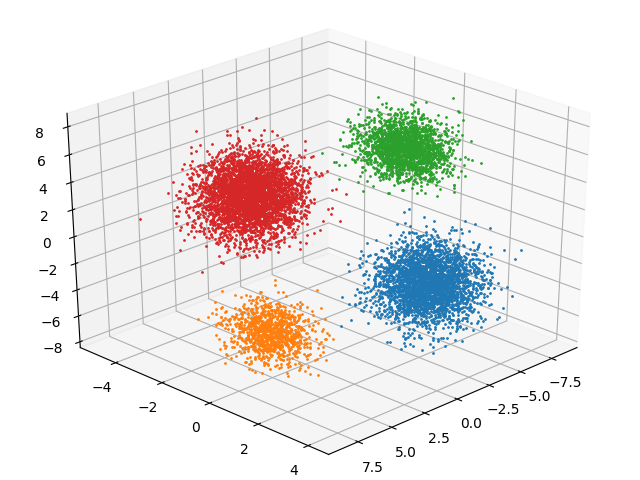
\includegraphics[width=0.6\linewidth]{./OMLkHtQWay.png}
\caption{$K=4$のEMアルゴリズムによる分類結果}
\label{fig:result}
\end{figure}

\end{document}
